\documentclass[reprint,amsmath,amssymb,aps,prl,groupedaddress,nofootinbib,superscriptaddress]{revtex4-1}
\usepackage{graphicx,xcolor,tikz}
\usepackage{amsthm,amssymb,amsmath,dsfont,braket}
\usepackage{bm}
\usepackage[hidelinks,pagebackref=false,pdfnewwindow=true]{hyperref} 
\usepackage{epstopdf,psfrag}
\usepackage{relsize,amsbsy}
\usepackage[export]{adjustbox}

\DeclareMathOperator{\sgn}{sgn}
\DeclareMathOperator{\tr}{Tr}
\DeclareMathOperator{\re}{Re}
\DeclareMathOperator{\im}{Im}

\newcommand{\dd}{\partial}
\newcommand{\1}{\mathds{1}}

\newcommand{\mac}{\mathcal}
\newcommand{\ms}{Majorana spinon }
\newcommand{\mss}{Majorana spinons }
\newcommand{\mssns}{Majorana spinons}
\newcommand{\hh}{harmonic honeycomb }
\newcommand{\HH}{Harmonic Honeycomb }
\newcommand{\Hs}[1]{\mbox{$\mathcal{H}$-$#1$}}
\newcommand{\zt}{\mathbb{Z}_2}

\begin{document}
		
	\title{Landau-level Raman peaks of Kitaev spinons under strain  
		}
		\author{Brent Perreault}
		\affiliation{\small School of Physics and Astronomy, University of Minnesota, Minneapolis, Minnesota 55455, USA}
		%	\email[]{perre035@umn.edu}
		%	\homepage[]{https://www.physics.umn.edu/people/perreault.html}
		%	
	%	\author{Johannes Knolle}
	%	\affiliation{\small Department of Physics, Cavendish Laboratory, JJ Thomson Avenue, Cambridge CB3 0HE, U.K.}
%		%	
%		\author{Natalia B. Perkins}
%		%	
%		\author{F. J. Burnell}
%		\affiliation{\small School of Physics and Astronomy, University of Minnesota, Minneapolis, Minnesota 55455, USA}
%		
		\date{\today} 
		
		\begin{abstract}	
			abstract
		\end{abstract}
		
\maketitle		

\graphicspath{{Figures/}}

{\it Introduction.} 
blah blah blah. SLs, Landau levels, JKK systems, Raman, ...

It was known for long before the discovery of graphene that free electrons on the honeycomb lattice would host Landau levels with a square-root dispersion \cite{Rammal85}. That strain induces effective gauge fields at linear order has been known for many years as well. Recently, effective gauge fields by strain were shown to lead to Landau level peaks in the density of states (DOS) of graphene.\cite{Vozmediano10,...} Analogously, Landau levels have been demonstrated in the Kitaev honeycomb model \cite{Rachel15}. Raman scattering should be able to probe the Landau-level peaks from the spinon DOS, which we demonstrate here with an explicit calculation.



{\it The Kitaev model.} %300 words 
We write the Kitaev honeycomb spin model as\cite{Kitaev06}
\begin{align}\label{H}
{H}_K &= \sum_{\left<ij\right>^\alpha} J^\alpha \sigma^\alpha_i \sigma^\alpha_j ,
\end{align}
where there is only one spin component interacting on each bond, with that component determined by the bond orientation. The solution given by Kitaev decomposes spins into a product of Majorana fermions by $\sigma^\alpha_j = i b^\alpha_j c_j$ to give 
\begin{align}\label{H2}
{H}_K &= \sum_{\left<ij\right>^\alpha} J^\alpha u_{\left<ij\right>^\alpha} c_i c_j,
\end{align}
where $u_{\left<ij\right>^\alpha} = i b_i^\alpha b_j^\alpha$ are conserved $Z_2$ gauge variables in the resultant theory. Since the gauge fluxes are gapped and conserved we can focus on the zero-flux ground-state gauge configuration gauged by $u_{\left<ij\right>^\alpha} = 1$ leaving a quadratic Hamiltonian in the dispersing $c$ Majorana spinons. Moreover, the Raman operator $R$ for this type of system realized as a Mott insulator also conserves fluxes so that dynamics can be considered entirely within the spinons.

In the absence of strain the Hamiltonian matrix of the honeycomb lattice reads
\begin{align}
\mathrm{H}_{\mathbf k} &= \frac{i}{2} \left( \begin{array}{cc}\label{HCH}
0 & \Gamma_{\mathbf k} \\
-\Gamma_{\mathbf k}^* & 0 \\
\end{array} \right) \hspace{0.4cm}
\Gamma_{\mathbf k} = J^z + J^x e^{ik_1} + J^y e^{ik_2} 
\end{align} 
where $\mathbf{c}_{\mathbf k}^T = (c_{A,{\mathbf k}},c_{B,{\mathbf k} })$, and we have chosen units such that the bond length is unity in the absence of strain so that $k_i = {\mathbf k}\cdot{\mathbf a}_i = (\sqrt{3}k_x \pm 3k_y)/2$.
The spectrum $\epsilon_k = 2|\Gamma_k|$ is identical to that of graphene with $J$ taking the place of a hopping parameter; gapless with a linear dispersion about two Dirac points $k_1 = -k_2 = \pm 2\pi/3$. 

{\it Strain-induced gauge fields.}
The strain field modifies the parameters $J$ in Eq.~(\ref{H}) by making the virtual hopping between sites stronger (weaker) for atoms that are closer together (further apart). At lowest order \cite{Rachel15} 
\begin{align}
\delta J_{ij}^\alpha / J &= - \beta \left( |\vec{\delta}_{ij}| - 1 \right) \approx -2\beta (\vec{\delta}_0 \cdot \vec{\nabla})(\vec{u}\cdot \vec{\delta}_0) , % = \vec{\delta}_0 + C(\vec{u}({R}_i) - \vec{u}({R}_j)),
\end{align}
where $\delta_0$ is the lattice vector in the absence of strain,  $\vec{u} = \vec{R}_j' - \vec{R}_j$ is the strain field, and $\vec{\delta}_{ij} = \vec{R}_i' - \vec{R}_j'$ is the strained lattice vector. Here $\beta \equiv -\frac{\partial \ln J}{\partial \ln \delta}$ is the magnetic Gr\"uneisen parameter \cite{White65}. Typical values for this parameter in a typical exchange setting are around $10$ \cite{Bloch66,Johnson74}. However, the origin of the Kitaev model in a Jackeli-Khaliullin-Kitaev (JKK) system \cite{Jackeli09} is significantly different making this parameter much more difficult to estimate. Based on recent electronic structure calculations it has been suggested that $\beta$ is negative for the Kitaev interaction in RuCl$_3$, indicating that it grows with tensile strain (stretch) while the competing interactions decay \cite{Kim16}, due to the changing Ru-Cl bond angles while that distance stays fixed. The results of Ref. \cite{Kim16} present indirect evidence, however, making a quantitative estimate difficult to extract from their data. A more focused ab initio calculation might help determine the correct value of $\beta$ for the strain engineering discussed below. 

%A reliable determination of the Gr\"uneisen parameter is a prerequisite of strain engineering for this model. For a realization in terms of a Jackeli-Khaliullin-Kitaev (JKK) system based on $t_{2g}$ orbitals $J$ is derived in terms of a super-exchange that involves an effective hopping $t$ from one transition-metal (TM) site to another mediated by oxygens. First, not that $J \sim t^2/U$ and $t \sim t_o^2 / \Delta_{\text{ch}} $ where $t_o$ is the hopping amplitude to an oxygen and $\Delta_{\text{ch}}$ is the charge transfer gap. Second, since the oxygen are placed at the corners of octahedra around TM atoms, and those octahedra share edges, the oxygen-TM distance scales as $\delta/\sqrt{2}$. This leads to $\beta \sim 2 \sqrt{2} \beta_o $ where $\beta_o \equiv \frac{\partial \ln J}{\partial \ln \delta}$ is the electron Gr\"uneisen parameter for hopping between TM ions and oxygen sites. $\beta_o$ is expected to be of order one. It can be measured nearly directly by applying a uniform bulk strain on the sample and observing the relative change in the optical phonon peak positions in Raman. For graphene the carbon-carbon hopping has $\beta_{CC} \sim 2$ \cite{Cheng11}. 

% can additionally increase hopping between certain ones of these orbitals over others thereby introducing other terms in the Hamiltonian. Here we ignore these terms, which a suppressed by the flux gap, and focus only on the effect on the Kitaev term through the magnitude of $J$. Phenomenologically, for the Coulomb interaction the overlap between two bonding orbitals decays like $1/R$ so that $\frac{d\ln t}{d \ln R} = 3/2$, where $R$ is the inter-site distance. In a JKK system $J \sim T^2/U$ where $T \sim t^2/\Delta_{ch}$ in terms of the hopping $t$ between an oxygen and a transition metal ion and the charge transfer gap $\Delta_{ch}$. Then since the oxygen-TM distance grows like $dR \sim dr / \sqrt{2}$ where $r$ is the TM-TM distance, then $\beta_J \equiv \frac{d\ln J}{d \ln r} ~ 2 \sqrt{2} ~ 3$.

To first order around the Dirac point 
\begin{align}
\delta \Gamma = \delta J^z + \delta J^x e^{i\frac{2\pi}{3}} + \delta J^y e^{-i\frac{2\pi}{3}}.
\end{align}
If we identify the effective gauge field as in % $\delta \Gamma = A^x - i A^y$ we find  
 %We will continue now by writing the Schroedinger equation for this Hamiltonian in a continuum-limit. 
%Continuing, 
\begin{align}
H_{\pm}(\mathbf{k}) =  i \frac{3}{2} J
\left(\begin{array}{cc}
0 & \mp i\partial_x + \partial_y - iA_x - A_y  \\
-c.c. & 0
\end{array}\right),
\end{align}
we find that $[A_x,A_y] = \beta [ {u_{xx}-u_{yy}} , 2u_{xy}]$ \cite{Vozmediano10}, where $u_{\alpha \beta} = \left[\partial_\alpha u_\beta + \partial_\alpha u_\beta \right]/2$. % and $v_f = |\partial_k \Gamma_k|_{k=0} = 3t/2$. 
This gives the effective out-of-plane magnetic field \cite{Zhu15}
%$$\gamma = B 3 \sqrt{3}/2 = \sqrt{3} \beta [-2 \partial_x u_{xy} - \partial_y (u_{xx}-u_{yy})]. $$
\begin{align}\label{B}
B = \beta \left[2\partial_x u_{xy} - \partial_y \left(u_{xx}-u_{yy}\right)\right].
\end{align}
%where $A=3\sqrt{3}/2 a^2$.


{\it Landau levels.} If $B$ is uniform, we can use the Landau gauge $\mathbf{A} = B(0,x)$ to write the Hamiltonian as
\begin{align}\label{LG}
H_{\pm}(\mathbf{k}) = i \frac{3}{2} J
\left(\begin{array}{cc}
0 & \mp i\partial_x + ik_y + B x \\
-c.c. & 0
\end{array}\right).
\end{align}
We can solve for the eigenvectors of Eq.~(\ref{LG}) can be solved as a harmonic oscillator by defining the raising and lowering operators
\begin{align}
\hat{a} = \frac{1}{\sqrt{2}} (\partial_\xi + \xi), \ \ \hat{a}^\dagger = \frac{1}{\sqrt{2}} (-\partial_\xi + \xi),
\end{align}
with the shifted coordinate $\xi = \sqrt{|B|} x + k_y/\sqrt{|B|}$. Then if we write $\psi(x,y) = \exp(ik_y y) \phi(y)$ so that $\partial_{k_y} \phi = 0$ the Schroedinger equation takes the form
\begin{align}
\frac{3}{2} J \sqrt{|B|}
\left(\begin{array}{cc}
0 & \hat{a} \\
\hat{a}^\dagger & 0
\end{array}\right) \phi(\xi) = E \phi(\xi).
\end{align}   
In terms of the eigenfunctions $\varphi_n$ of the harmonic oscillator, the eigenvectors are \cite{Neto09,McClure56}
\begin{align}
\phi_{n,\pm}(\xi) &= 
\left(\begin{array}{c}
\varphi_{n-1}(\xi)  \\
\pm \varphi_n(\xi)
\end{array}\right) ,\ \ n = 0,1,2,... \\
\varepsilon_{n,\pm}& = \pm \frac{3}{2} J \sqrt{|B|} \sqrt{n}, \label{spectrum}
\end{align} 
where each level is degenerate with a state for every value of the quantum number $k_y$. 

A peculiarity of the Bogoliubov-deGennes form of the Majorana Hamiltonian is that the physical eigenstates appear twice in the eigenstates of the Hamiltonian matrix,\cite{Blaizot86} related by particle-hole symmetry $\psi_{k_y,n} = \psi^\dagger_{-k_y,n}$, with opposite eigenvalues corresponding to half the excitation energy. This is particularly important when we use the Schroedinger picture to describe a low-energy theory. Away from zero-energy we can remedy this by simply taking only the positive-energy eigenstates with the appropriate energy, while dropping the negative-energy ones. Therefore, based on the spectrum of Eq.~(\ref{spectrum}), we expect that the low energy states, which are near the Dirac points, are redistributed to flat bands at the energies $E_{n} = 3 J \sqrt{|B|} \sqrt{n}$ where $n = 0,1,2,...$ so that we expect the density of states to develop peaks at those energies.

{\it Raman scattering.} 
The coupling of Raman scattering to the fractionalized quasiparticles of the Kitaev model has been discussed by our group the past few years \cite{Knolle14-2,Perreault15,Perreault16-1,Perreault16-2}. In short, the Raman operators turn out to be analogous to the Hamiltonian with the coupling of a given term augmented by factors determined by the angle between the light-polarization and the bonds involved in the corresponding electronic process. The Raman intensity is a correlation function of such events, each tracking the dynamics of two spinons in the Kitaev fractionalization.

Given a strain pattern that does not affect the symmetries of the Hamiltonian there are two independent, non-zero Raman scattering intensities available to experiment, which are a function of $\omega$, but not $k$ due to the large laser spot typically used. These are the intensities in the $A_{1g}=E_{g}$ channel and the $A_{2g}$ channel, where the latter one appears only when the incoming photon frequency is nearly relevant with the minimal Mott gap \cite{Perreault16-1}.

{\it Raman matrix elements.}
It was shown in our previous works that the latter channel picks up the zero-energy flat band states due to the inability of the former to create a pair of flat-band states. We demonstrate here that these two-spinon operators couple to distinct sets of Landau-level pairs. 

To proceed we write out the eigenstates in the continuum picture developed above, but now in terms of the low-energy fermionic operators that diagonalize the Hamiltonian, which was initially fermionic. 
%In terms of fermionic quasiparticles, in the presence of the magnetic field we have found that the low-energy modes near the Dirac point are split into highly degenerate Landau levels with energy $E_{n} = 3 t \sqrt{|B|} \sqrt{n}$ where $n = 0,1,2,...$ We now wish to write this in terms of the low-energy fermionic operators that diagonalize the Hamiltonian, which was initially fermionic.
Then the Hamiltonian takes the form%To fit with this picture the Hamiltonian must be quadratic in fermionic quasiparticles as well, and therefore the Landau level ladder operator must be as well.
\begin{align}
H &= \sum_{k_y,n} E_{n} \psi^\dagger_{k_y,n} \psi_{k_y,n},
%\mathbf{a} &\equiv \sum_{k_y,n} \psi^\dagger_{k_y,n+1} \psi_{k_y,n}
\end{align} 
where we define a lowering operator in terms of its sublattice parts by
\begin{align}
\psi_{k_y,n} &= \psi_{k_y,n}^A + \psi_{k_y,n}^B \\
\psi_{k_y,n}^A &= \sum_{x,y} e^{ik_y y} \varphi_{n-1}(\xi(x,k_y)) c_{x,y}^A \\
\psi_{k_y,n}^B &= \sum_{x,y} e^{ik_y y} \varphi_{n}(\xi(x,k_y)) c_{x,y}^B.
\end{align}
%Then the harmonic oscillator (HO) ladder operators can be written as 
%\begin{align}
%(a^A)^\dagger &= \sum_{k_y,n} \left(\psi^A_{k_y,n+1}\right)^\dagger \psi_{k_y,n}^A \\
%(a^B)^\dagger &= \sum_{k_y,n} \left(\psi^A_{k_y,n+1}\right)^\dagger \psi_{k_y,n}^B
%\end{align}
%Consider the Raman operator in the $yy$ channel. In the absence of strain it takes the form of 
%\begin{align}
%\mathrm{R}_{\mathbf k} &= \frac{i}{4} \left( \begin{array}{cc}\label{Ryy}
%0 & 1 \\
%-1 & 0 \\
%\end{array} \right) + H_k/2,
%\end{align}
%where we can ignore the part that goes like the Hamiltonian since it does not create any excitations.
%To write this in terms of the diagonal operators $\psi_{k_y,n}^{A/B}$ we can invert the eigenvector relation to find
%\begin{align}
%c^a_{x,y} = \sum_{k_y} e^{-ik_y y} \sum_{} 
%\end{align}
To evaluate the Raman operator in the diagonal basis we may compute the overlap of the Raman operator $R^{yy} = \sum_{x,y} i c^A_{x,y} c^B_{x,y} /2$, representative of the $A_{1g}$ channel, with a product wavefunction $\psi^\dagger_{k_y,n} \psi^\dagger_{-k_y,m}$, where the form of $k_y$ is dictated by the translation invariance of $R$. Expanding the product this is 
\begin{align}
R^{yy}_{m,n,k_y} &= (-i/2) \sum_{x} \varphi_m^*(\xi(k_y,x)) \varphi_{n-1}^*(\xi(-k_y,x)) + h.c. \nonumber
\\ &= \pm \sum_{x} \varphi_m^*(\xi(k_y,x)) \varphi_{n-1}(\xi(k_y,x))  + h.c. \nonumber \\ & = 0, \quad \ \ \text{unless m = n-1},
\end{align}
where in the second line we used the particle-hole symmetry. In the last line we used the orthogonality of the HO eigenstates $\varphi_n$. This leads to the expectation that this operator creates pairs of excitations: one with energy $E_n$ and the other with $E_{n-1}$, for a total energy of $3 J \sqrt{|B|} (\sqrt{n}+\sqrt{n-1})$, with the off-by-one rule coming from the form of the wavefunctions in terms of HO wavefunctions whose level is different by a unit. A similar argument works for the other symmetric channels in the continuum limit, which are all proportional to $\sum_{x,y} i c^A_{x,y} c^B_{x,y}$ in the continuum limit due to their locality and sublattice symmetry.  

On the other hand, the operator $R^{[xy]}$ is dominated by a term $\sim \sum_{x,y} i c^A_{x,y} c^A_{x,y}$. A similar analysis gives \begin{align}
R^{[xy]}_{m,n,k_y} \propto \braket{\phi_m|\phi_n},
\end{align}
which requires that $m=n$ for the two excitations created by the Raman operator in the $A_{2g}$ channel. This leads one to expect to see peaks in this Raman channel at the energies $2 E_n$.


{\it Results.} 
We follow the Refs.~\cite{Guinea10,Amal13,Rachel15} to study a honeycomb flake, strained in a way that preserves the $S_6$ lattice symmetry. With the strain% to model a strained honeycomb flake. We take $x$ and $y$ to be the positions of a lattice site without any strain (the base configuration makes a perfect honeycomb), measured in units of $a_0$, the lattice constant (the distance between two NN sites). We then write
\begin{align}
\vec{u}(x,y) = C(2xy,x^2-y^2)
\end{align}
it is simple to check from Eq.~(\ref{B}) that one obtains a uniform effective magnetic field with magnitude $B = -8 \beta C$. This pattern can be visualized as in Fig. \ref{honeycomb_flake}.

We construct the honeycomb flake as $r$ layers of honeycombs placed around an initial single one as in Fig. \ref{honeycomb_flake} \cite{Rachel15}. We choose to characterize the strain by the total amount of strain along the directions of maximal stretching and compression $s = \frac{\delta L}{L} = \sqrt{3}C(r+\frac{1}{2})$ so that $B \approx \frac{4\beta}{\sqrt{3}r}s$. For linear elasticity to hold we need $s \ll \frac{\sqrt{3}}{2\beta}$. 

We take $\beta = 10$. For this case the optimal parameters are strains of $1$-$4$\% and system sizes of $r = 25$-$50$ unit cells. In RuCl$_3$ an unstrained honeycomb is about $6$\AA \ so that such flakes would have diameters of $30$-$60$nm. 
We find that for the magnetic field to be strong enough at to create noticeable Landau levels at these system sizes it needs to be on the order of $B\approx 0.03$ and that the levels appear/disappear sharply near that value. With increasing system size the maximum value of $B$ decays with $1/r$, putting constraints on how large the honeycomb flake can be. This is in competition with the need to have a large enough system to get a spectrum that is not too noisy. 


% 
%
%as the fundamental strain so that $\vec{U} = C \vec{u}$ to describes the displacement vector of the strain, where $C$ is a dimensionless constant fixes the rate of strain growth from the center of the flake to the edge. In the strained lattice, then, the position of each site is $\vec{R}' = \vec{R} + \vec{U}({R})$. 
%
%In the presence of this strain the couplings are taken to change linearly in the amount they stretched. This gives
%% that can be characterized by two parameters $\beta$ and $C$.
%%For the model, see their Eqs.~(3) and (4). In particular, let me write
%\begin{align}
%J_{ij}^\alpha &= J \left[1  - \beta \left(  |\vec{\delta}_{ij}| - 1 \right) \right], \nonumber\\ \vec{\delta} &= \vec{R}_i' - \vec{R}_j' = \vec{\delta}_0 + C(\vec{u}({R}_i) - \vec{u}({R}_j)).
%\end{align}
%In Ref. \cite{Rachel15} they mistakenly suggest that there is only one essential parameter. Due to their confusion they do not give enough information to know what model they used, making difficult to make a direct comparison. [I have tried emailing the authors about this to no avail.]
%
%I build the lattice layer-by-layer as suggested by Fig. S1 in Ref. \cite{Rachel15} except that I number the first honeycomb as $r=0$. 

%{\it Results}
%In Fig. \ref{fig:stretch1} I show the 

\begin{figure}
	\centering
	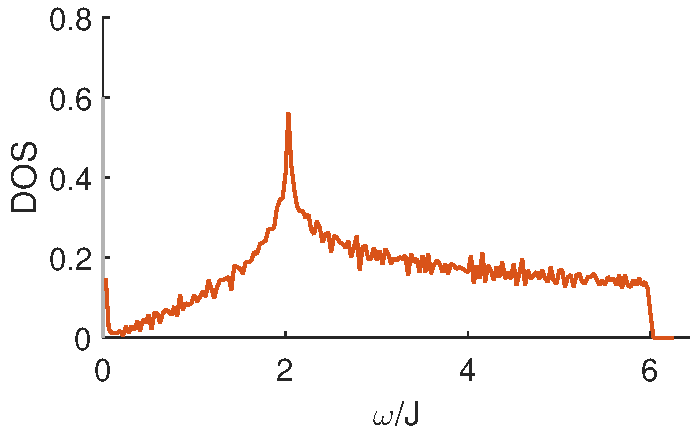
\includegraphics[width=0.9\linewidth]{stretch_DOS_rmax_50_b_10_c_0_p_0-eps-converted-to.pdf} 
	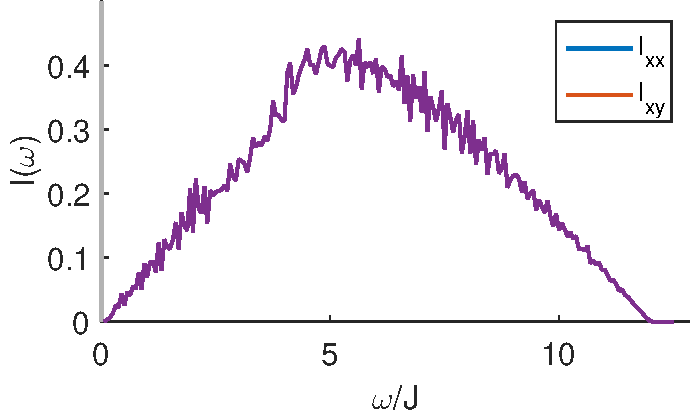
\includegraphics[width=0.9\linewidth]{stretch_I2_rmax_50_b_10_c_0_p_0-eps-converted-to.pdf} 
	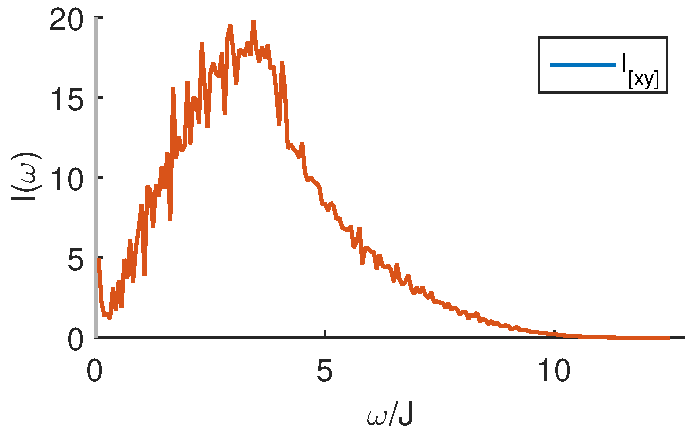
\includegraphics[width=0.9\linewidth]{stretch_I3_rmax_50_b_10_c_0_p_0-eps-converted-to.pdf}
	\caption{The DOS and all possible Raman correlation functions in the absence of strain with $r=50$ corresponding to a $6*(50+1)^2 = 15606$ sites.  This looks very much like the thermodynamic limit with some fuzziness due to the small system size.} % ($6*(50+1)^2 = 15606$ sites). The difference is that there is a large peak in the DOS at zero energy due to an edge mode. Such an edge mode can be understood similarly to the Fermi line in of the hyper- (Harmonic) honeycomb lattice(s). This peak is not in the (symmetric) Raman. It is significantly more coding to construct the second neighbor lattice required to create the resonant Raman operator, so I just haven't done it. However, I expect the low-energy peak to be noticeable there. This question would be technically easier to answer in a strip configuration, which I plan to do soon.}
	\label{fig:stretch1}
\end{figure}

\begin{figure}
	\centering
	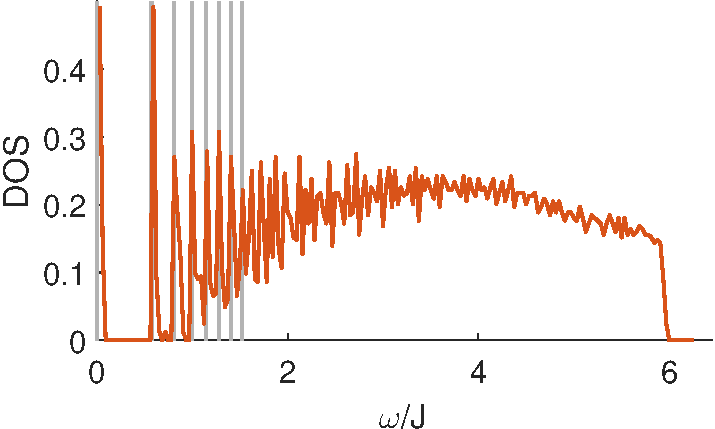
\includegraphics[width=0.9\linewidth]{stretch_DOS_rmax_50_b_10_c_40_p_0-eps-converted-to.pdf} 
	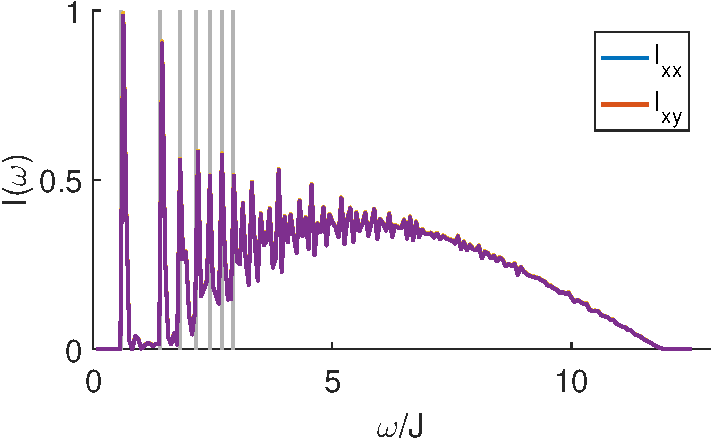
\includegraphics[width=0.9\linewidth]{stretch_I2_rmax_50_b_10_c_40_p_0-eps-converted-to.pdf} 
	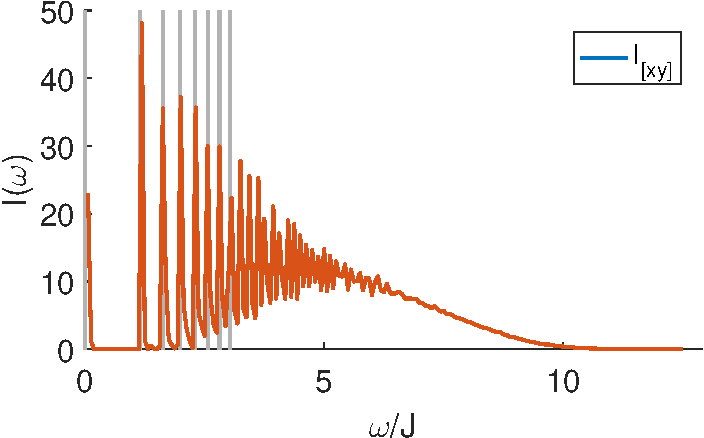
\includegraphics[width=0.9\linewidth]{stretch_I3_rmax_50_b_10_c_40_p_0-eps-converted-to.pdf}
	\caption{Here I have introduced strain: $r=50$, $\beta=10$, $s=0.04$, or $4$\% maximum total strain. % I see Landau levels as well as they could be seen in Fig. 2 or Ref.~\cite{Rachel15}. Note that the zero-energy peak is still absent. Notice that the LF-relationship has been broken, but the symmetry relationships remain \cite{Perreault16-1,Perreault16-2}. 
	The gray lines represent $E_0 \sqrt{n}$, $E_0 (\sqrt{n} + \sqrt{n+1})$ and $E_0 2 \sqrt{n}$ respectively, where $E_0$ is predicted based on the values of $\beta$ and $s$.}
	\label{fig:stretch2}
\end{figure}

\begin{figure}
	\centering
	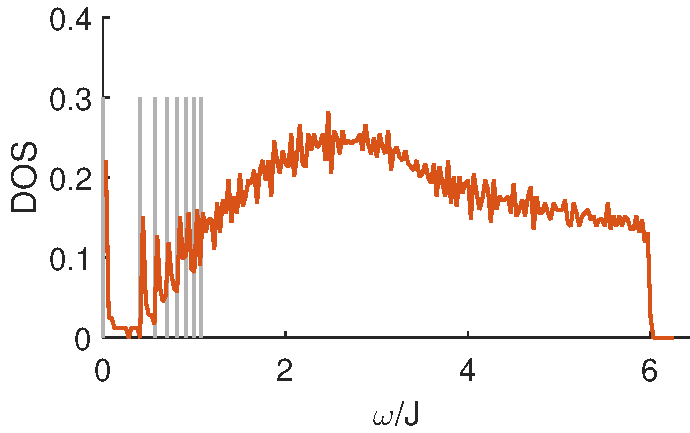
\includegraphics[width=0.9\linewidth]{stretch_DOS_rmax_50_b_10_c_20_p_0-eps-converted-to.pdf} 
	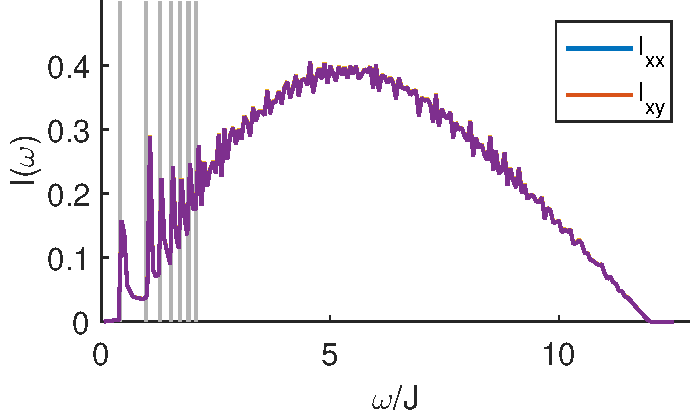
\includegraphics[width=0.9\linewidth]{stretch_I2_rmax_50_b_10_c_20_p_0-eps-converted-to.pdf} 
	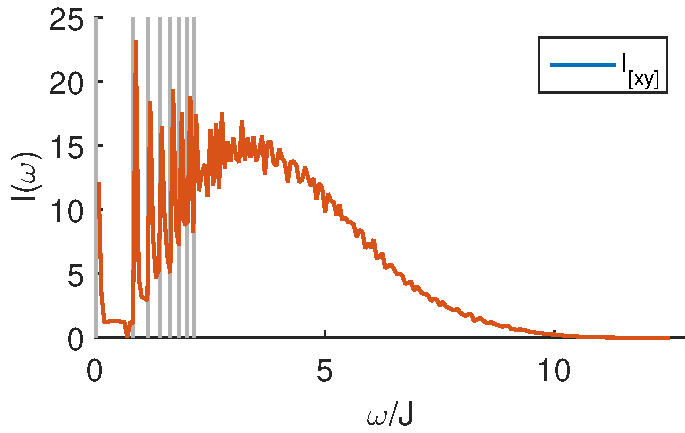
\includegraphics[width=0.9\linewidth]{stretch_I3_rmax_50_b_10_c_20_p_0-eps-converted-to.pdf}
	\caption{Here I have introduced strain: $r=50$, $\beta=10$, $s=0.02$, or $2$\% maximum total strain. }% I see Landau levels as well as they could be seen in Fig. 2 or Ref.~\cite{Rachel15}. Note that the zero-energy peak is still absent. Notice that the LF-relationship has been broken, but the symmetry relationships remain \cite{Perreault16-1,Perreault16-2}. 
		%The gray lines represent $E_0 \sqrt{n}$, $E_0 (\sqrt{n} + \sqrt{n+1})$ and $E_0 2 \sqrt{n}$ respectively, where $E_0$ is predicted based on the values of $\beta$ and $s$.}
	\label{fig:stretch3}
\end{figure}

\begin{figure}
	\centering
	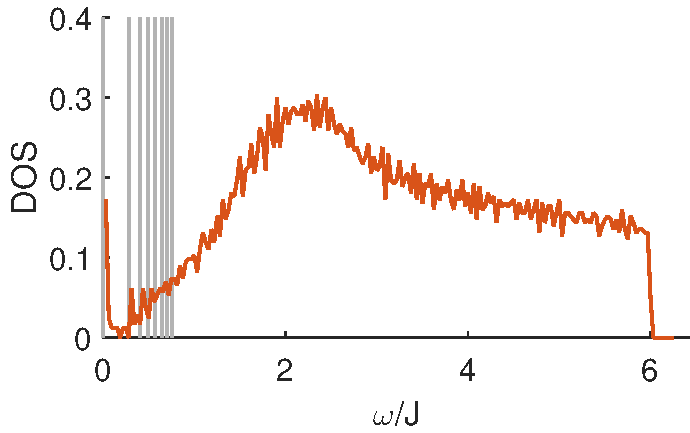
\includegraphics[width=0.9\linewidth]{stretch_DOS_rmax_50_b_10_c_10_p_0-eps-converted-to.pdf} 
	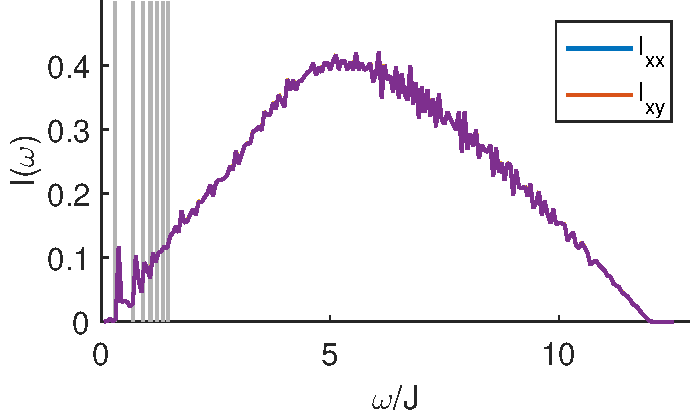
\includegraphics[width=0.9\linewidth]{stretch_I2_rmax_50_b_10_c_10_p_0-eps-converted-to.pdf} 
	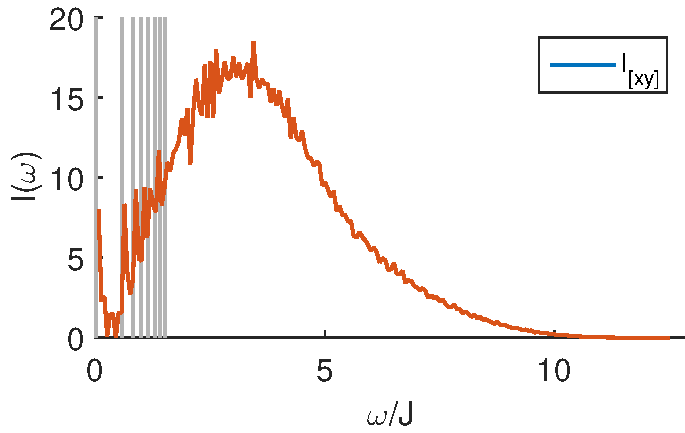
\includegraphics[width=0.9\linewidth]{stretch_I3_rmax_50_b_10_c_10_p_0-eps-converted-to.pdf}
	\caption{Here I have introduced strain: $r=50$, $\beta=10$, $s=0.01$, or $1$\% maximum total strain. } % I see Landau levels as well as they could be seen in Fig. 2 or Ref.~\cite{Rachel15}. Note that the zero-energy peak is still absent. Notice that the LF-relationship has been broken, but the symmetry relationships remain \cite{Perreault16-1,Perreault16-2}. 
		%The gray lines represent $E_0 \sqrt{n}$, $E_0 (\sqrt{n} + \sqrt{n+1})$ and $E_0 2 \sqrt{n}$ respectively, where $E_0$ is predicted based on the values of $\beta$ and $s$.}
	\label{fig:stretch4}
\end{figure}



{\it Discussion.}







 
%{\it The SVD trick for sublattice-symmetric Majoranas and the Raman weights.} I just put this here to remember to write this down later. 




\section*{Acknowledgements}
Kenneth Burch, Stephan Rachel

\bibliography{strain_refs}

%\onecolumngrid
%\appendix
%
%\section{Supplementary Material}

\end{document}